Sistem elektronik robot hexapod membagi fungsi antara STM32F407 dan Jetson Nano
secara terstruktur. STM32F407 (modul M.2) mengendalikan servo kaki, sedangkan
Jetson Nano menangani komputasi kinematika dan perencanaan gerak lengan 6-DOF\@.
Untuk meningkatkan kestabilan dan mengurangi interferensi, catu daya dipisah
menjadi dua jalur: satu untuk servo dan satu untuk sistem kontrol, guna
mengisolasi rangkaian daya tinggi dari logika dan meningkatkan keandalan sistem.

\subsection{\emph{Power Board}} 
\label{sec:driver_board}
\begin{figure} [H] \centering
  % Nama dari file gambar yang diinputkan
  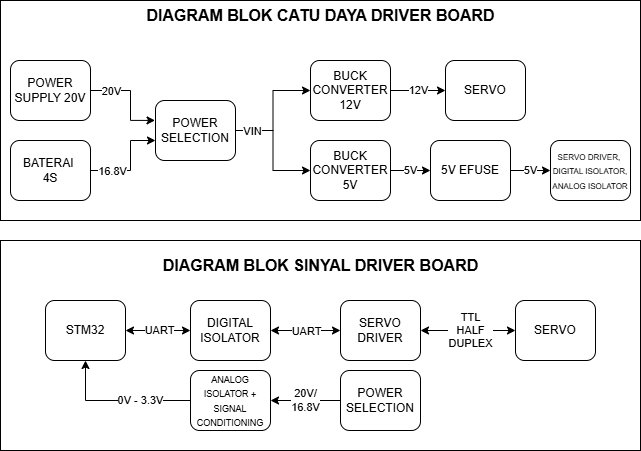
\includegraphics[scale=0.6]{gambar/PCB_Driver.png}
  % Keterangan gambar yang diinputkan
  \caption{Diagram Blok PCB \emph{PCB} \emph{power}}
  % Label referensi dari gambar yang diinputkan
  \label{fig:catu_daya}
\end{figure}

\emph{power board} merupakan papan sirkuit cetak (PCB) yang dirancang khusus
untuk menjalankan dan memberikan catu daya kepada motor servo. Pada gambar
\ref{fig:catu_daya} sistem catu daya untuk menyalakan servo dan rangkaian
lainnya memiliki dua sumber catu daya utama, yaitu baterai 4S dan \emph{power
supply} 20V. Kedua sumber tersebut dihubungkan dengan rangkaian \emph{power
selection} yang berfungsi untuk memilih sumber catu daya yang akan digunakan.

\begin{figure} [H] \centering
  % Nama dari file gambar yang diinputkan
  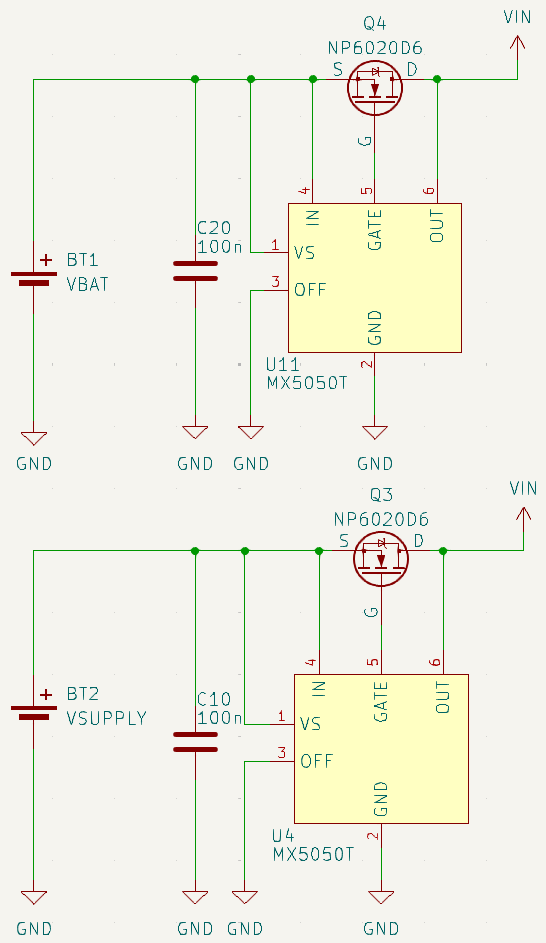
\includegraphics[scale=0.5]{gambar/Ideal_Diode.png}
  % Keterangan gambar yang diinputkan
  \caption{Rangkaian \emph{Power Selection}}
  % Label referensi dari gambar yang diinputkan
  \label{fig:power_selection}
\end{figure}
Rangkaian \emph{power selection} pada gambar \ref{fig:power_selection}
menggunakan \emph{NMOSFET} yang dikontrol melalui \emph{ mosfet}.
Rangkaian ini dapat diibaratkan sebagai gerbang logika OR yang menggunakan dioda.
Sumber catu daya yang memiliki tegangan lebih tinggi akan mengalirkan arus ke
beban, sedangkan sumber catu daya yang memiliki tegangan lebih rendah akan
terputus dari beban. Tujuan dilakukan pemilihan sumber catu daya ini adalah
untuk mempermudah saat melakukan pergantian baterai tanpa harus mematikan sistem.

Bagian selanjutnya merupakan rangkaian buck converter. Pada PCB ini, terdapat dua buah buck 
converter yang digunakan. Buck converter pertama berfungsi untuk menurunkan sumber tegangan
menjadi 12V, yang digunakan untuk menyuplai catu daya servo. Kemudian buck converter kedua 
berfungsi untuk menurunkan sumber tegangan menjadi 5V, yang digunakan sebagai suplai catu daya
untuk rangkaian lainnya.
\newpage

\begin{figure} [H] \centering
  % Nama dari file gambar yang diinputkan
  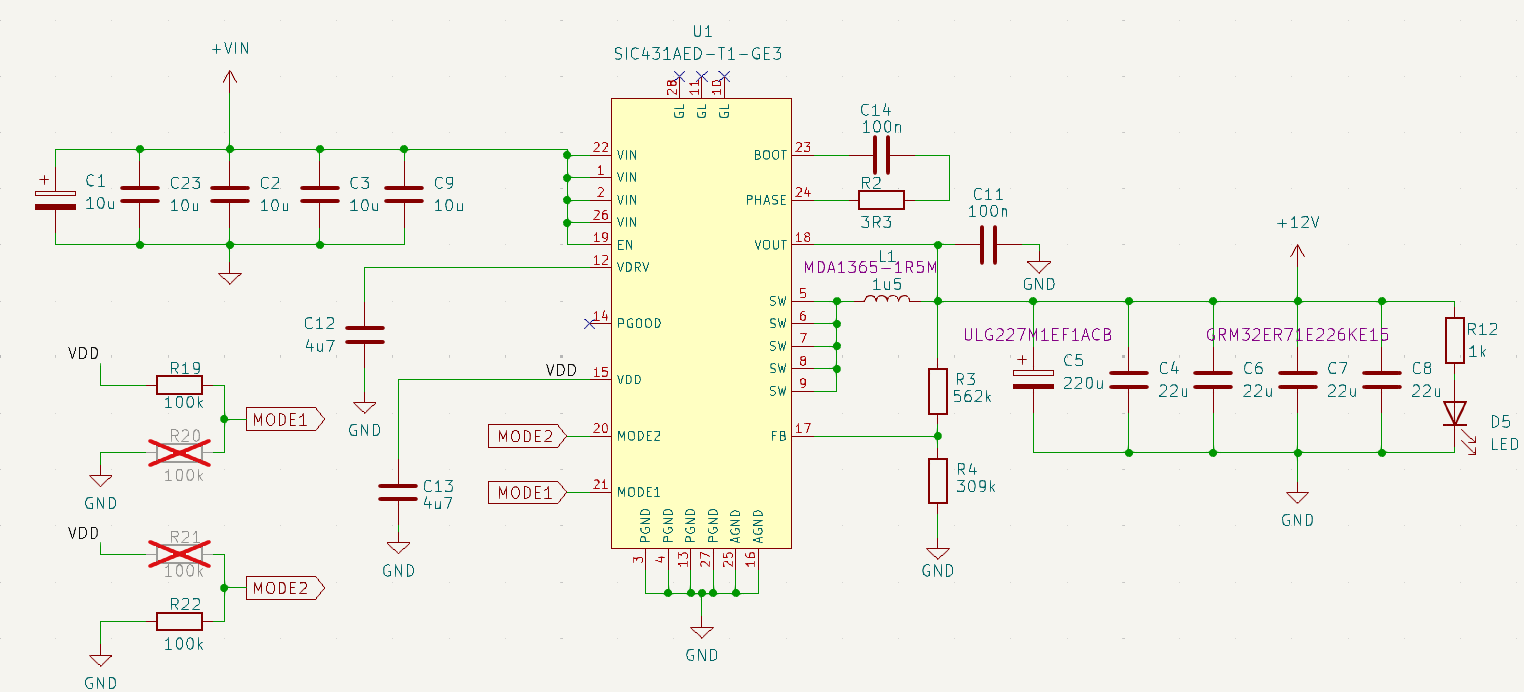
\includegraphics[scale=0.38]{gambar/Buck_12V.png}
  % Keterangan gambar yang diinputkan
  \caption{Rangkaian Buck Converter 12V}
  % Label referensi dari gambar yang diinputkan
  \label{fig:buck_converter}
\end{figure}
Rangkaian buck converter pada gambar \ref{fig:buck_converter} menggunakan \emph{SIC431AED}
sebagai \emph{switching regulator} yang memiliki efisiensi tinggi. Penggunaan \emph{SIC431AED}
sebagai regulator buck converter karena dapat menyuplai arus hingga 24A.\emph{SIC431AED}
sudah dilengkapi dengan mosfet internal yang dapat mengurangi jumlah komponen yang digunakan. input
minimal dari buck converter ini adalah 1,1*Voutput, yang mana jika outpunya adalah 12V, maka tegangan
input minimalnya adalah 13,2V (dibawah rentang kerja baterai 4S, yaitu 14,8V s.d. 16,8V)\parencite{SIC431}.

\begin{figure} [H] \centering
  % Nama dari file gambar yang diinputkan
  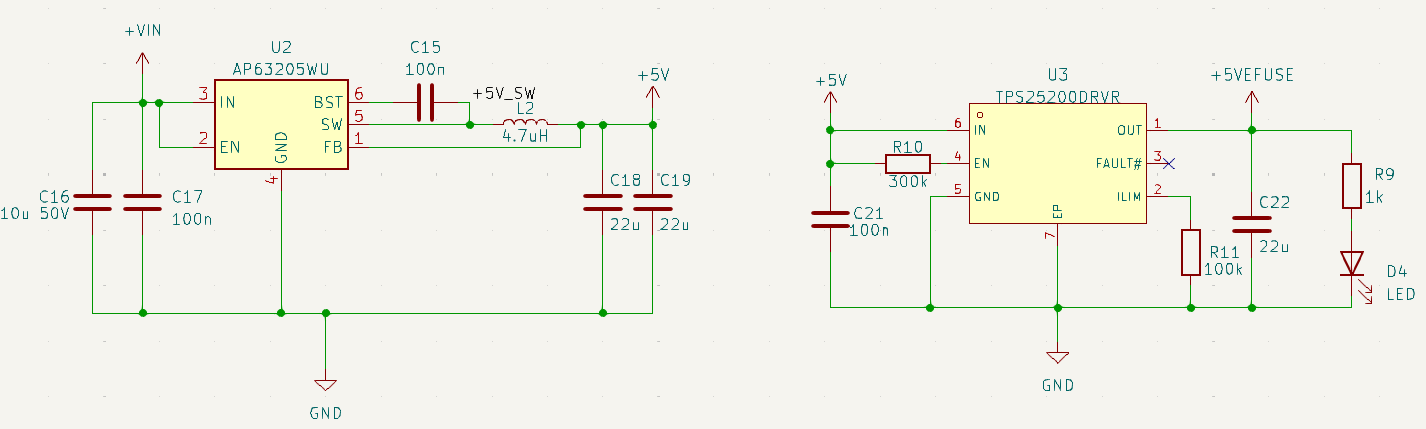
\includegraphics[scale=0.4]{gambar/Buck_5V.png}
  % Keterangan gambar yang diinputkan
  \caption{Rangkaian Buck Converter 5V}
  % Label referensi dari gambar yang diinputkan
  \label{fig:buck_converter_5v}
\end{figure}

Untuk suplai catu daya 5V, digunakan buck converter \emph{AP63205}. Pemilihan
\emph{AP63205} sebagai buck converter untuk suplai 5V karena ukurannya yang
kecil dan beban yang menggunakan catu daya 5V tidak besar. \emph{AP63205} dapat
menyuplai arus hingga 2A dengan efesiensi hingga 95\%. \parencite{AP63205}.  

Pada gambar \ref{fig:buck_converter_5v}, sebelum output buck converter dihubungkan ke beban,
terdapat rangkaian proteksi untuk mencegah kerusakan pada komponen yang  menggunakan catu daya 5V.
Rangkaian proteksi ini menggunkana \emph{eFuse} yang berfungsi untuk menjaga agar arus yang 
mengalir ke beban tidak melebihi batas yang telah ditentukan (1A) jika terjadi \emph{short circuit}
pada beban. Penentuan batas arus ditentukan melalui pemilihan resistor yang terhubung pada
pin \emph{ilim} pada \emph{eFuse}. \parencite{TPS25200}

Untuk memberikan informasi mengenai sumber catu daya yang digunakan dan besar tegangan
baterai pada seiring waktu, digunakan sebuah rangkaian monitoring sumber catu daya. Rangkaian
ini terdiri dari \emph{voltage divider} untuk menurunkan tegangan baterai/suplai,\emph{analog 
isolator} yang berfungsi untuk mengisolasi sinyal tegangan baterai/suplai. Output dari analog
isolator ini dihubungkan ke \emph{ADC} pada mikrokontroler STM32F407 untuk dibaca
sebagai informasi tegangan baterai/suplai.

\begin{figure} [H] \centering
  % Nama dari file gambar yang diinputkan
  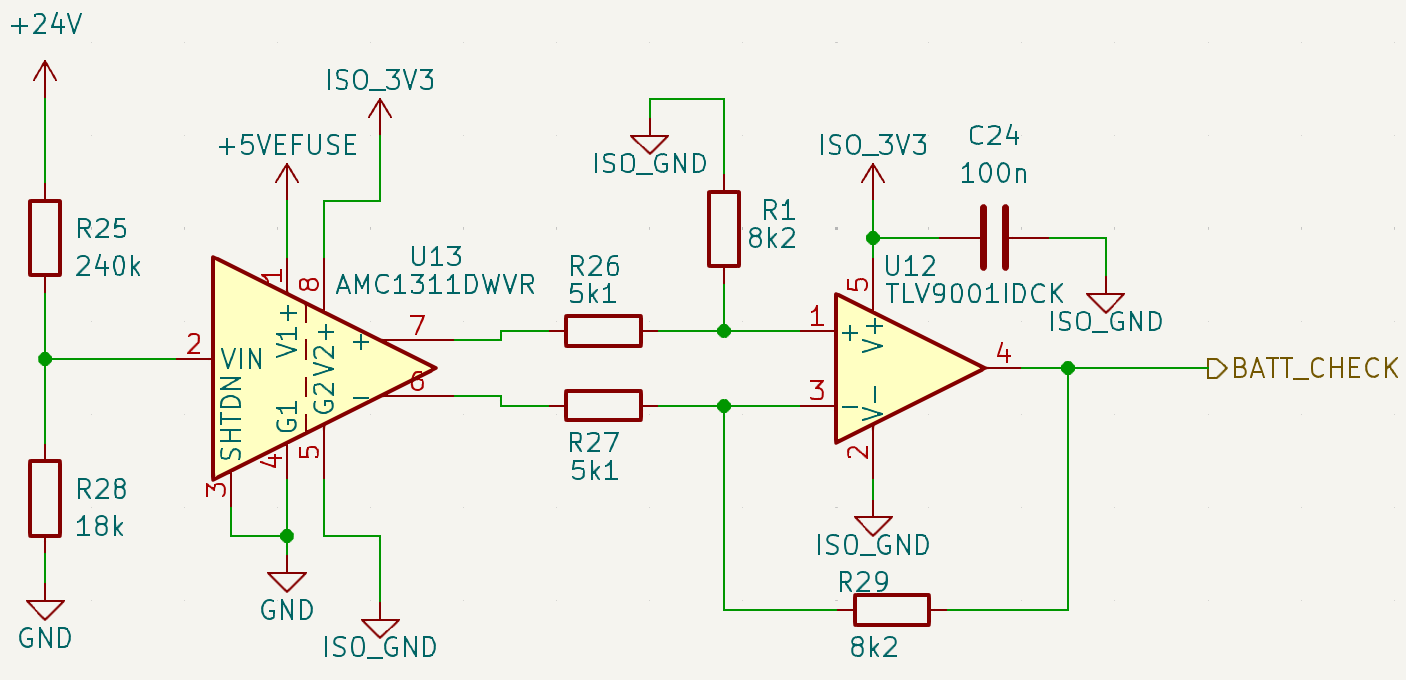
\includegraphics[scale=0.4]{gambar/Vsense.png}
  % Keterangan gambar yang diinputkan
  \caption{Rangkaian monitoring sumber catu daya}
  % Label referensi dari gambar yang diinputkan
  \label{fig:vsense}
\end{figure}

Rangkaian monitoring sumber catu daya pada gambar \ref{fig:vsense} menggunakan
\emph{voltage divider} untuk menurunkan tegangan baterai/suplai ke tegangan 2V 
menyesuaikan spesisfikasi dari analog isolator (\emph{AMC1311}). Walaupun pada
implementasi normal robot ini hanya dioperasikan dengan sumber baterai 4S
(maksimum $\pm$16,8~V) atau catu daya eksternal 20~V, perancangan pembagi
tegangan tetap dilakukan berdasarkan asumsi tegangan masukan 30~V. Pendekatan
ini dimaksudkan sebagai faktor pengaman (\emph{safety margin}) untuk
mengantisipasi kondisi tak terduga, seperti lonjakan tegangan, kesalahan
konfigurasi catu daya, atau penggunaan sumber tegangan yang lebih tinggi pada
masa pengujian dan pengembangan.

Output dari AMC1311 merupakan sinyal diferensial yang kemudian diubah menjadi
sinyal tunggal menggunakan \emph{differential amplifier} (\emph{TLV9001}) dengan
gain sebesar 1.6 untuk menyesuaikan rentang tegangan yang dapat dibaca oleh ADC
pada mikrokontroler STM32F407 (0--3.3~V). Rangkaian ini berfungsi sebagai tahap
\emph{signal conditioning} untuk mengkonversi sinyal diferensial menjadi sinyal
tunggal dengan level tegangan yang sesuai standar ADC mikrokontroler. Selain itu,
pemilihan penguatan dan konfigurasi penguat dilakukan agar linearitas dan
resolusi ADC dapat dimanfaatkan secara optimal.

Bagian terakhir dari PCB ini adalah rangkaian komunikasi servo. Seperti yang
sudah disampaikan sebelumnya, jenis servo yang digunakan adalah \emph{smart
servo} yang berkomunikasi menggunakan \emph{TTL Half-Duplex}. Oleh karena itu 
diperlukan sebuah rangkaian konversi yang mengubah sinyal komunikasi serial
dari STM32 menjadi menjadi \emph{TTL Half-Duplex} sehingga memungkinkan komunikasi 
dengan servo.

\begin{figure} [H] \centering
  % Nama dari file gambar yang diinputkan
  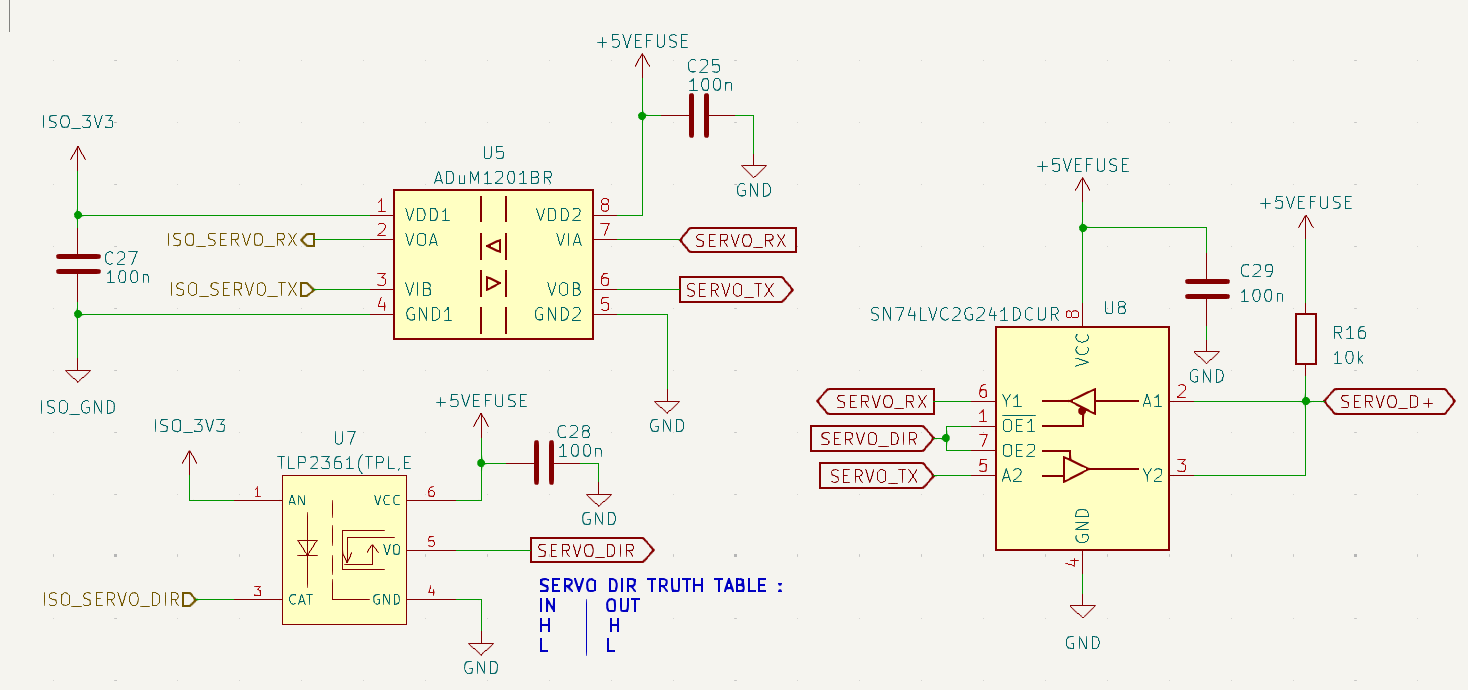
\includegraphics[scale=0.4]{gambar/Driver_Servo.png}
  % Keterangan gambar yang diinputkan
  \caption{Rangkaian Komunikasi Servo}
  % Label referensi dari gambar yang diinputkan
  \label{fig:komunikasi_servo} 
\end{figure}

Gambar \ref{fig:komunikasi_servo} merupakan sistem komunikasi terisolasi yang dirancang 
untuk mengendalikan arah dan pertukaran data antara STM32 dan servo. Isolasi
galvanik diterapkan menggunakan isolator digital \emph{ADuM1201} untuk sinyal data
dan optokopler \emph{TLP2361} untuk arah komunikasi, sehingga sisi kontrol dan
sisi daya servo tetap terpisah secara elektrik. Data dikirim dan diterima melalui
jalur komunikasi serial, dan dikonversi menjadi komunikasi TTL half-duplex
menggunakan buffer dua kanal \emph{SN74LVC2G241}. IC ini menggabungkan jalur TX dan RX
menjadi satu jalur data dua arah, dengan arah komunikasi dikendalikan oleh
sinyal logika dari mikrokontroler. 

\subsection{Modul M.2 STM32F407}
Pada perancangan robot hexapod ini, mikrokontroler STM32F407 dipilih untuk 
menjalankan setiap servo pada robot. STM32F407 dibuat dalam bentuk modul M.2
2230 yang bertujuan untuk memungkinkan integrasi langsung antara STM32 dan
Jetson Nano pada satu papan sirkuit cetak (PCB), sehingga ukuran sistem
elektronik secara keseluruhan dapat dibuat lebih kecil dan ringkas.
\\

\begin{figure}[H]
  \centering
  \begin{subfigure}{0.47\textwidth}
    \centering
    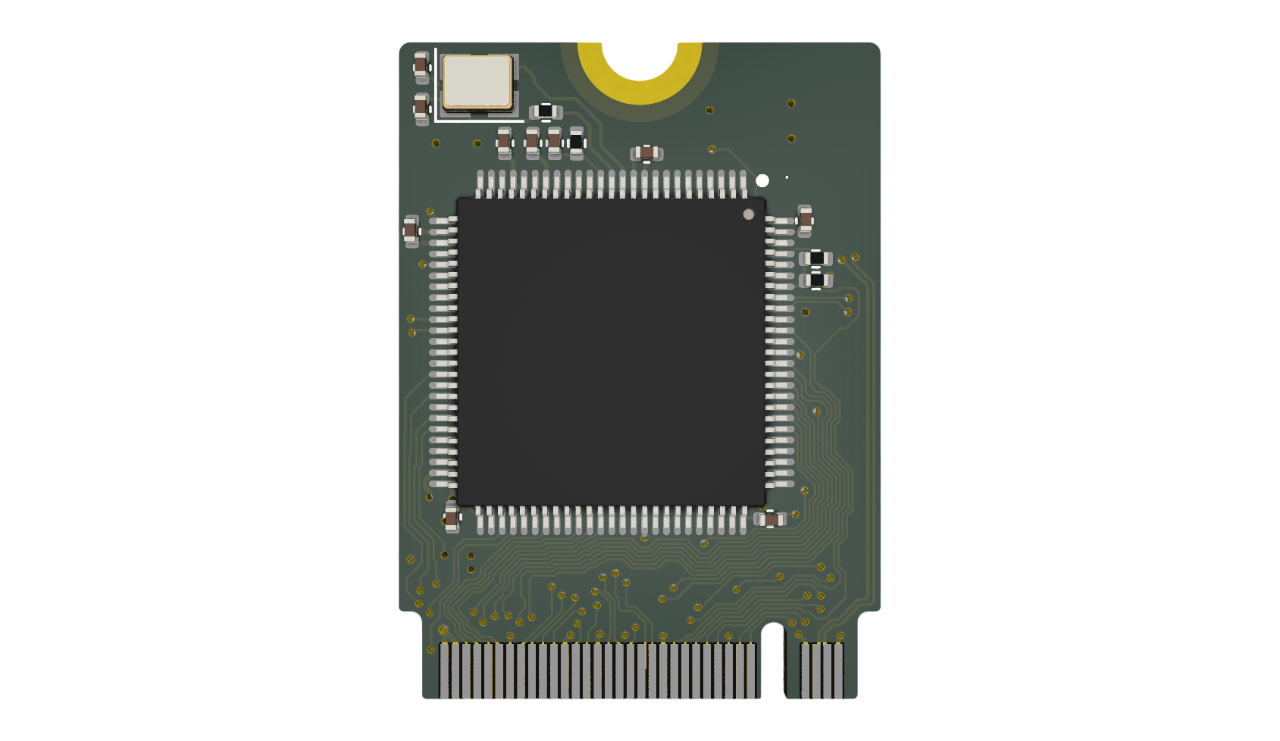
\includegraphics[width=\textwidth]{gambar/STM_BOT.png}
    \caption{Tampak Bawah Modul STM32}
    \label{fig:Desain}
  \end{subfigure}
  \hfill
  \begin{subfigure}{0.47\textwidth}
    \centering
    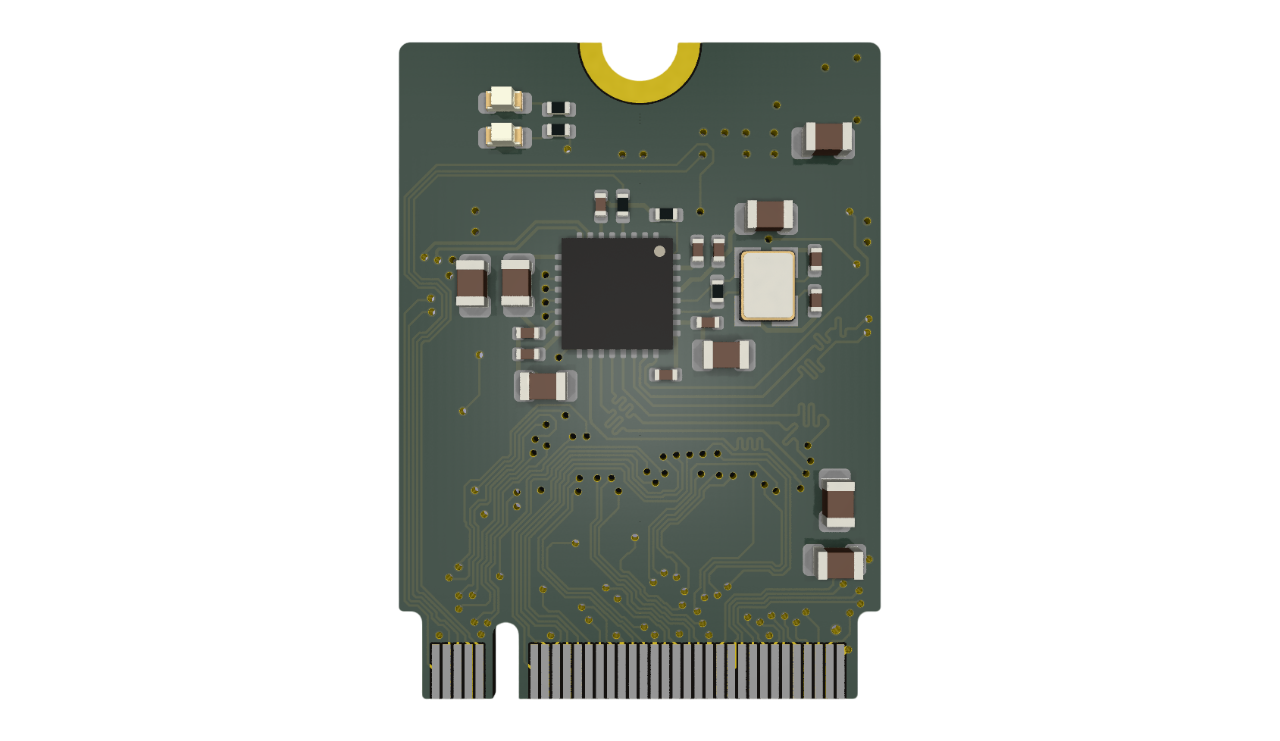
\includegraphics[width=\textwidth]{gambar/STM_TOP.png}
    \caption{Tampak Atas Modul STM32}
    \label{fig:layout}
  \end{subfigure}
  \caption{Desain PCB Modul STM32}
  \label{fig:PCB_}
\end{figure}

Untuk memungkinkan komunikasi berkecepatan tinggi dengan sistem komputasi Jetson
Nano, modul ini dilengkapi dengan chip USB PHY USB3300 yang mengimplementasikan
protokol USB 2.0 High Speed (480 Mbps). Integrasi USB3300 diperlukan karena
mikrokontroler STM32F407 hanya menyediakan antarmuka USB \emph{Full Speed} secara
bawaan. Dengan penambahan USB3300, mikrokontroler dapat berfungsi sebagai
perangkat USB berkecepatan tinggi, yang dibutuhkan untuk mempercepat transfer
data antarperangkat, khususnya pada aplikasi yang bersifat responsif.

\begin{figure} [H] \centering
  % Nama dari file gambar yang diinputkan
  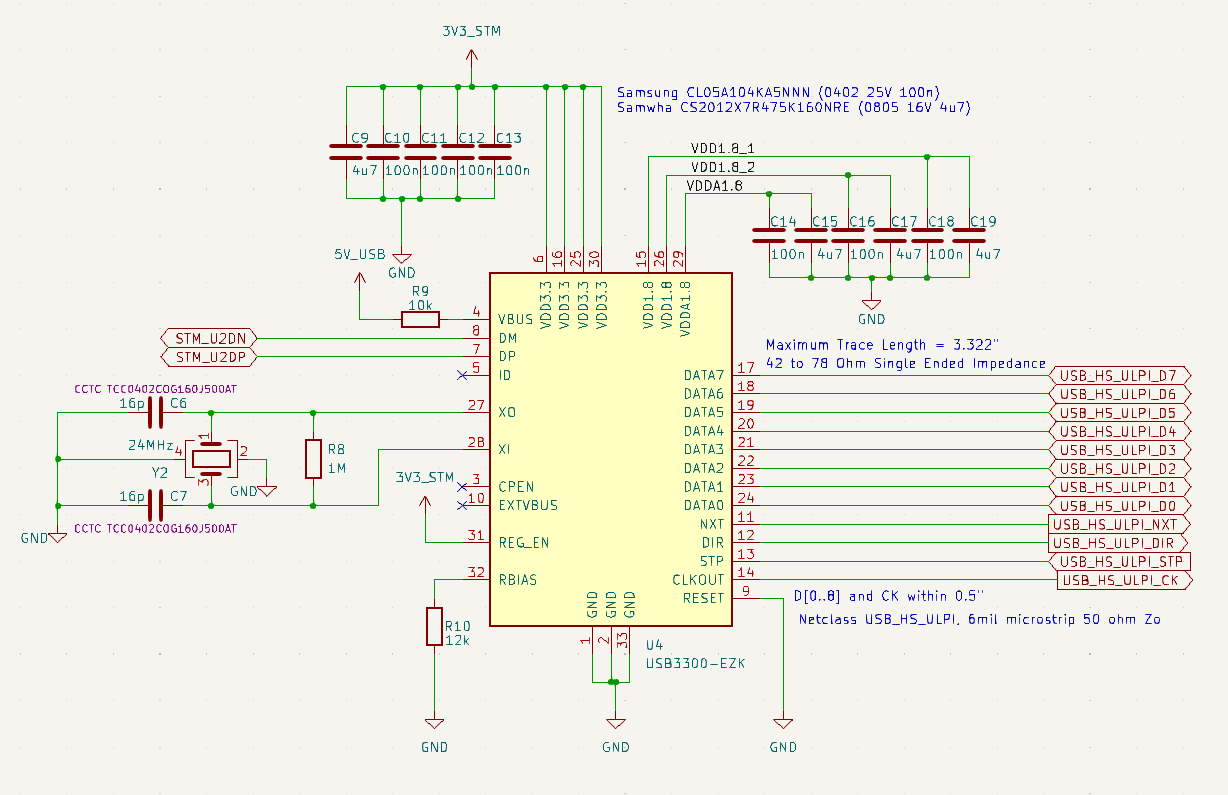
\includegraphics[scale=0.35]{gambar/Gambar_ULPI.png}
  % Keterangan gambar yang diinputkan
  \caption{Rangkaian USB3300}
  % Label referensi dari gambar yang diinputkan
  \label{fig:USB_ULPI}
\end{figure}

Modul ini menggunakan crystal oscillator 24 MHz sebagai sumber clock eksternal,
yang dihubungkan ke pin HSE (\emph{High Speed External}) pada STM32F407 untuk
menjamin kestabilan frekuensi operasional. Tegangan kerja modul adalah 3,3V,
yang disuplai dari sistem catu daya logika. Untuk mendukung performa sinyal dan
kestabilan sistem secara keseluruhan, desain PCB pada modul ini menggunakan enam
lapisan dengan susunan Signal-Ground-Power-Power-Ground-Signal. Stack-up ini
dirancang untuk meminimalkan rugi sinyal (\emph{signal integrity loss}),
mengurangi EMI (\emph{electromagnetic interference}), serta menjaga distribusi
daya yang stabil pada jalur internal.
\newpage

\subsection{\emph{Main Board}}
\begin{figure} [H] \centering
  % Nama dari file gambar yang diinputkan
  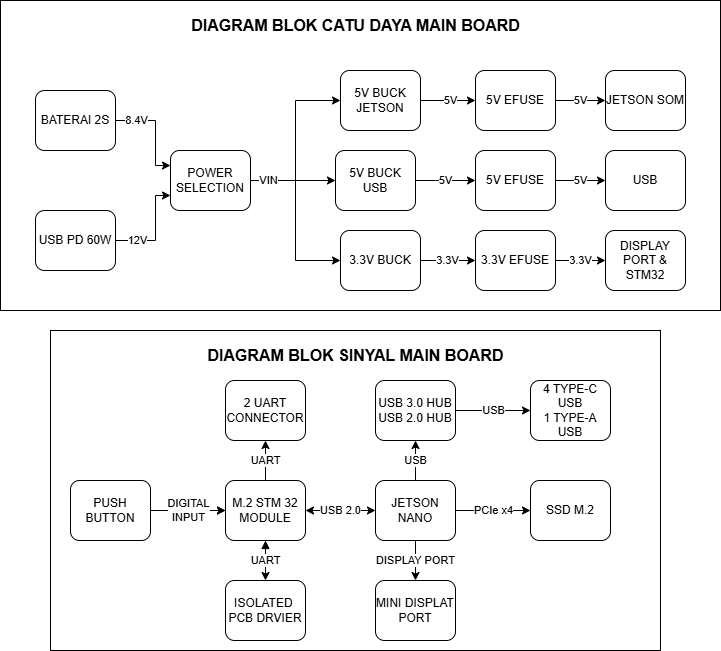
\includegraphics[scale=0.6]{gambar/Main_Board.drawio.png}
  % Keterangan gambar yang diinputkan
  \caption{Diagram Blok \emph{Main Board}}
  % Label referensi dari gambar yang diinputkan
  \label{fig:main_board}
\end{figure}

Main Board berfungsi sebagai pusat kendali utama yang menghubungkan STM32F407,
Jetson Nano, dan seluruh komponen pendukung lainnya. Modul STM32F407 dalam
bentuk M.2 bertugas mengatur komunikasi dengan servo pada kaki, lengan, dan
kepala robot, sedangkan Jetson Nano menangani perhitungan kinematika dan
perencanaan gerak. Komponen pendukung lainnya meliputi SSD NVMe sebagai media
penyimpanan utama, mini display port untuk koneksi ke layar eksternal, serta
empat port USB 3.0 untuk perangkat periferal. Terdapat port UART
yang terhubung ke STM32F407, beberapa push button sebagai input untuk
mengaktifkan sistem, dan berbagai fitur tambahan lainnya sebagai pelengkap pada 
main board ini (buzzer, LED indikator, dll).

Main board dapat diberi daya dari dua sumber, yaitu baterai 2S dan USB PD 60W
(12V 5A), yang secara otomatis dipilih melalui rangkaian power selection. 
Tegangan kemudian dikonversi oleh tiga buah buck converter menjadi 5V untuk
Jetson Nano, 5V untuk port USB, dan 3.3V untuk STM32 serta komponen lainnya.
Gambar \ref{fig:buck_main_board} memperlihatkan rangkaian buck converter
pada main board yang menggunakan IC TPS54821. Ketiga buck converter menggunakan tipe yang yang sama dan 
memiliki rangkaian yang hampir serupa. Yang menjadi pembeda adalah besar 
output tegangan yang dihasilkan yang diatur dari feedback resistor yang digunakan. 

\begin{figure} [H] \centering
  % Nama dari file gambar yang diinputkan
  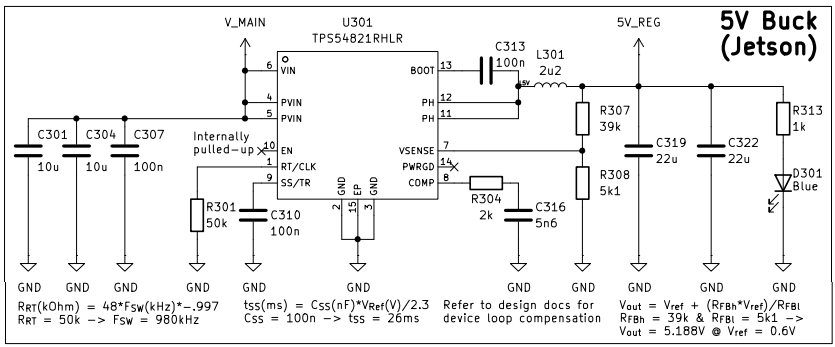
\includegraphics[scale=0.6]{gambar/Buck_Jetson_bk.png}
  % Keterangan gambar yang diinputkan
  \caption{\emph{Buck converter} pada \emph{main board}}
  % Label referensi dari gambar yang diinputkan
  \label{fig:buck_main_board}
\end{figure}
Sebelum dihubungkan ke seluruh sistem, setiap jalur sumber daya akan di proteksi oleh
rangkaian \emph{efuse}. Sama seperti \emph{power board} efuse yang digunakan berfungsi 
untuk mengatur arus yang keluar ke beban. Namun, tipe efuse yang digunakan berbeda. Pada 
\emph{main board} seluruh efuse menggunakan TPS259530DSGR. Jumlah arus yang dibatasi oleh
\emph{efuse} dapat diatur mulai dari 0.75A s.d. 4A dengan akurasi $ \pm $7.5\%.\parencite{TPS259530DSGR}

\begin{figure} [H] \centering
  % Nama dari file gambar yang diinputkan
  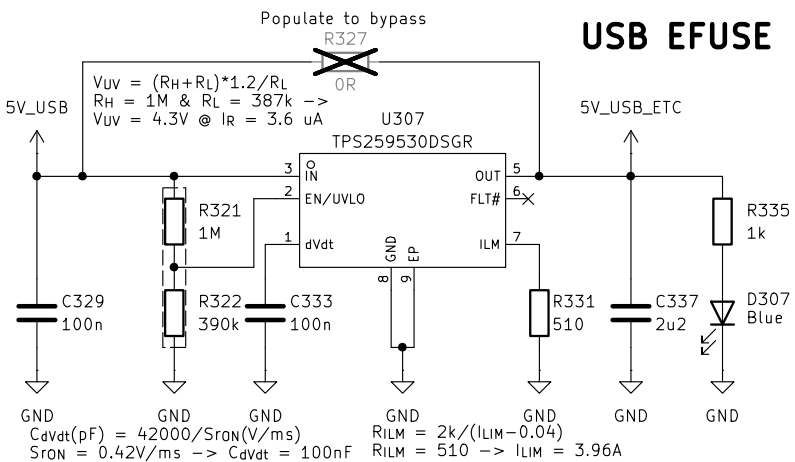
\includegraphics[scale=0.6]{gambar/Efuse_Mainboard_bk.png}
  % Keterangan gambar yang diinputkan
  \caption{\emph{Efuse} pada \emph{main board}}
  % Label referensi dari gambar yang diinputkan
  \label{fig:efuse_main_board}
\end{figure}

Terdapat total 6 buah rangkaian \emph{efuse} yang digunakan pada PCB ini (Jetson,
STM32, USB, SSD, M.2, dan \emph{display port}). Setiap \emph{efuse} diatur
besar arus limit-nya berdasarkan beban yang digunakan. Kemudian dari rangkaian
\ref{fig:efuse_main_board} Terdapat opsi untuk melakukan \emph{bypass} jika
terjadi masalah pada \emph{efuse} atau beban langsung dihubungkan ke buck
converter tanpa melalui \emph{efuse}.

Jetson Nano pada \textit{main board} ini menyediakan tiga buah port USB 2.0
\textit{host} dan satu port USB 3.0 \textit{host}. Untuk menambah jumlah port
USB yang tersedia, \textit{main board} ini dilengkapi dengan sebuah \textit{USB
hub} menggunakan \textit{UPD720210K8}. \textit{USB hub} tersebut memecah satu
port \textit{USB host} menjadi empat port USB. Keluaran dari
\textit{UPD720210K8} dihubungkan ke tiga port USB tipe-C dan satu port USB
tipe-A. Selain itu, terdapat \textit{FE1.1} yang merupakan \textit{USB hub}
khusus untuk USB 2.0. Salah satu port USB 2.0 \textit{host} dari Jetson Nano
dihubungkan ke \textit{FE1.1}, dan keluarannya dialirkan ke satu port USB tipe-C
serta ke modul STM32F407.

\begin{figure} [H] \centering
  % Nama dari file gambar yang diinputkan
  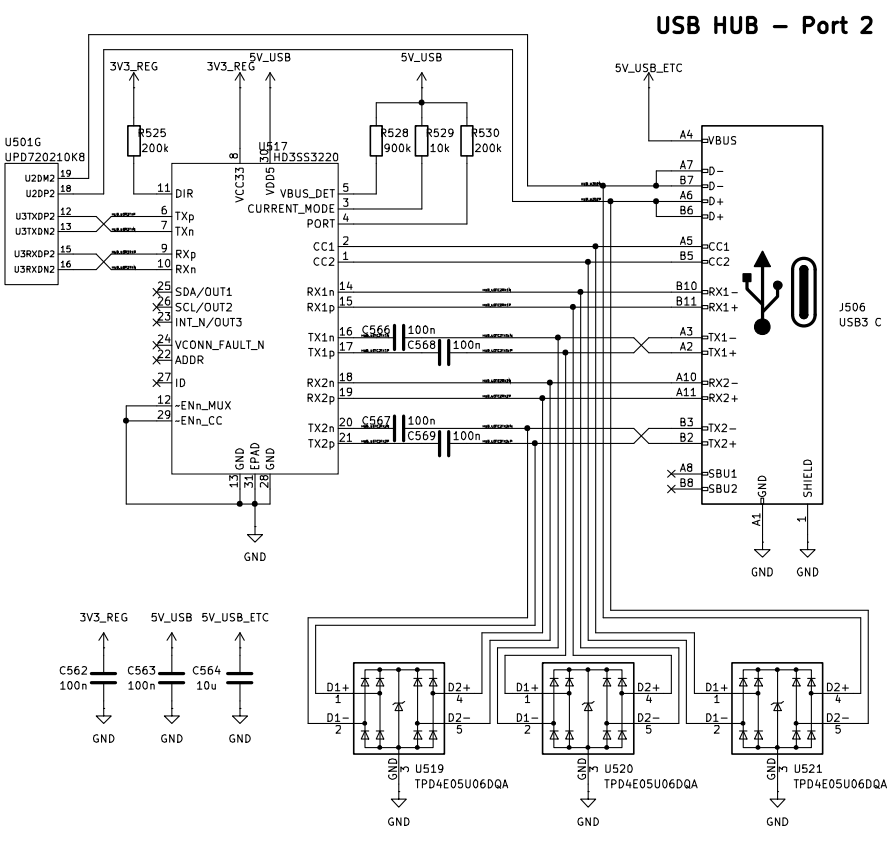
\includegraphics[scale=0.46]{gambar/USB_Port_bk.png}
  % Keterangan gambar yang diinputkan
  \caption{Port USB pada \emph{main board}}
  % Label referensi dari gambar yang diinputkan
  \label{fig:usb_main_board}
\end{figure}

Pada konektor USB Tipe-C dengan standar USB 3.0, diperlukan sebuah rangkaian
\textit{multiplexer} untuk mengatur jalur sinyal berkecepatan tinggi
(\textit{SuperSpeed}) yang bersifat diferensial. Hal ini disebabkan oleh
karakteristik konektor USB Tipe-C yang bersifat \textit{reversible}, sehingga
orientasi sambungan dapat berbeda-beda ketika perangkat dicolokkan. Tanpa adanya
\textit{multiplexer}, jalur \textit{SuperSpeed} tidak akan terhubung dengan
benar sesuai orientasi konektor, yang dapat menyebabkan penurunan kecepatan atau
kegagalan komunikasi. Oleh karena itu, pada \textit{main board} ini digunakan IC
\textit{HD3SS3220} sebagai \textit{USB SuperSpeed multiplexer} untuk secara
otomatis mengalihkan jalur TX/RX sesuai orientasi konektor USB Tipe-C, sekaligus
menjaga integritas sinyal agar sesuai dengan standar USB 3.0.

Selain itu, untuk melindungi jalur sinyal USB dari gangguan tegangan berlebih
akibat \textit{electrostatic discharge} (ESD), pada \textit{main board} ini
digunakan IC \texttt{TPD4E05U06DQA}. IC ini merupakan \textit{low-capacitance
ESD protection device} yang dirancang khusus untuk aplikasi berkecepatan tinggi
seperti USB 2.0/3.0. Dengan kapasitansi yang sangat rendah,
\texttt{TPD4E05U06DQA} mampu menjaga integritas sinyal diferensial USB sambil
memberikan proteksi terhadap lonjakan tegangan hingga tingkat \textit{IEC
61000-4-2} (±12kV \emph{Contact discharge} dan ±15kV \emph{Air-gap discharge} )
ESD. Pemasangan IC ini dilakukan sedekat mungkin dengan konektor USB sehingga
perlindungan maksimal dapat diberikan pada jalur D+/D– dan jalur
\textit{SuperSpeed} TX/RX.\parencite{TPD4E05U06DQA}

Konektor \textit{Mini DisplayPort} dan \textit{M.2 SSD} pada \textit{main board}
ini dirancang untuk meneruskan fungsi antarmuka Jetson Nano ke perangkat
eksternal. Jalur-jalur yang menghubungkan Jetson Nano dengan kedua konektor ini
bersifat langsung sesuai standar masing-masing antarmuka sehingga tidak
memerlukan rangkaian yang rumit.

\begin{figure} [H] \centering
  % Nama dari file gambar yang diinputkan
  \includegraphics[scale=0.33]{gambar/Mini_DP_bk.png}
  % Keterangan gambar yang diinputkan
  \caption{Port Mini DisplayPort pada \emph{main board}}
  % Label referensi dari gambar yang diinputkan
  \label{fig:mini_dp_main_board}
\end{figure}

\begin{figure} [H] \centering
  % Nama dari file gambar yang diinputkan
  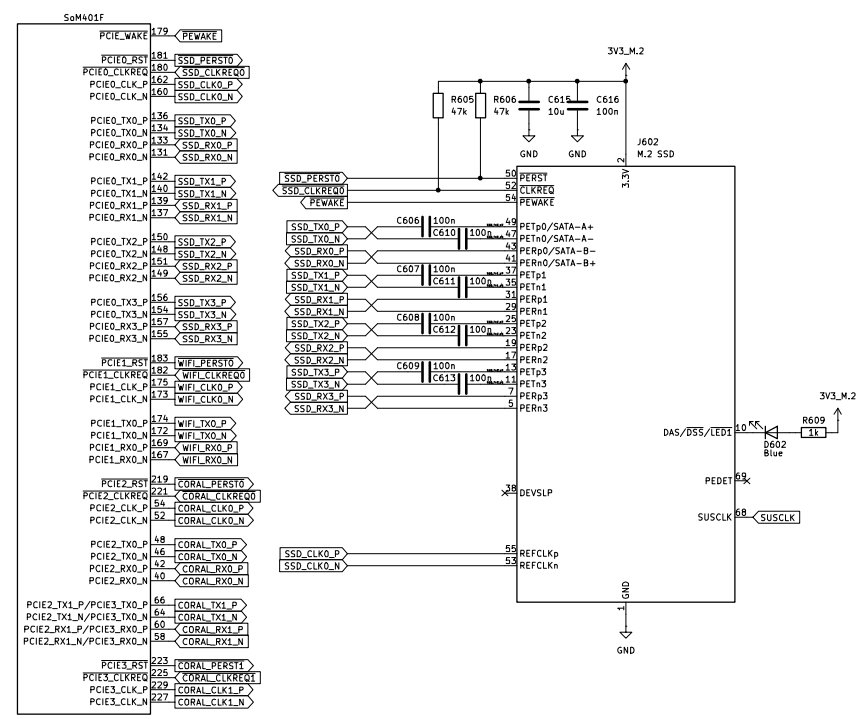
\includegraphics[scale=0.55]{gambar/SSD_bk.png}
  % Keterangan gambar yang diinputkan
  \caption{Port M.2 SSD pada \emph{main board}}
  % Label referensi dari gambar yang diinputkan
  \label{fig:ssd_main_board}
\end{figure}

Gambar~\ref{fig:mini_dp_main_board} memperlihatkan rancangan jalur \textit{Mini
DisplayPort} dan \textit{M.2 SSD} pada \textit{main board}. Kedua antarmuka ini
pada dasarnya merupakan perpanjangan jalur sinyal Jetson Nano ke konektor
eksternal sehingga tidak memerlukan sirkuit tambahan yang kompleks. Pada
\textit{Mini DisplayPort}, dipasang komponen proteksi ESD untuk melindungi jalur
berkecepatan tinggi dari lonjakan tegangan elektrostatik, sedangkan pada
\textit{M.2 SSD}, jalur PCIe langsung dihubungkan dari Jetson Nano ke slot
\textit{M.2} dengan penyesuaian impedansi sesuai standar untuk menjaga
integritas sinyal.

Bagian terakhir dari \textit{main board} adalah modul STM32F407. Modul STM32F407
dalam bentuk M.2 yang sudah dirancang sebelumnya, akan disatukan pada \emph{main board}.

\begin{figure} [H] \centering
  % Nama dari file gambar yang diinputkan
  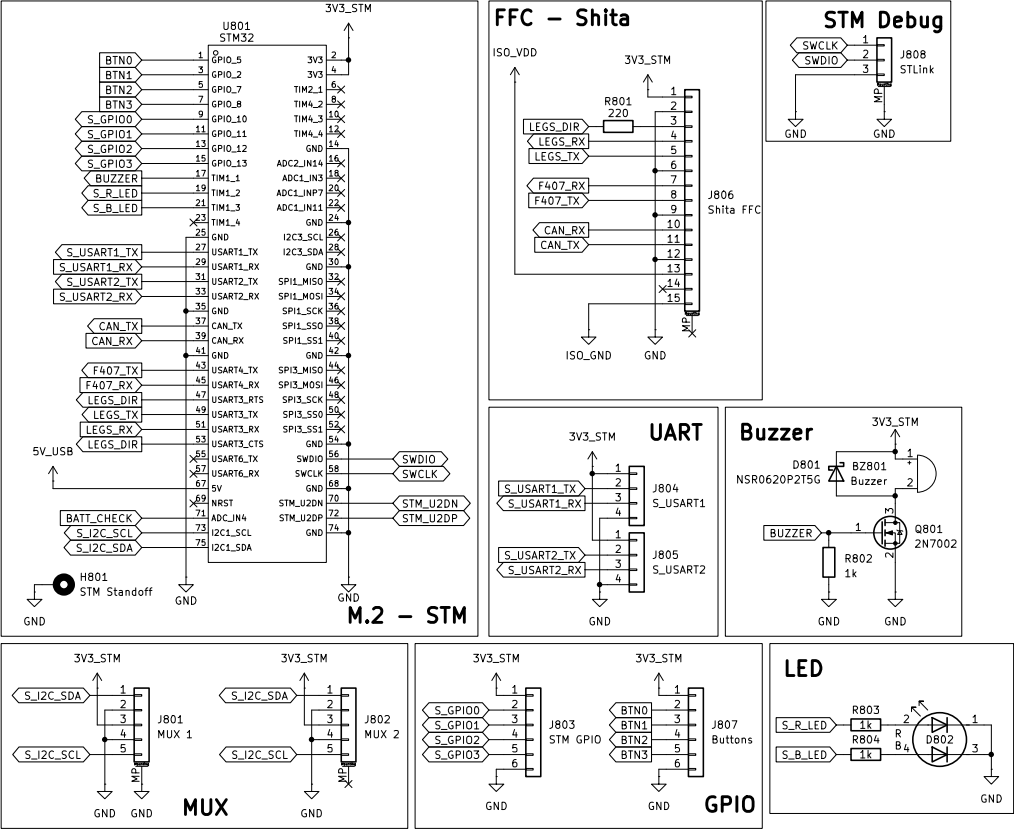
\includegraphics[scale=0.59]{gambar/skema_stm_main_board_bk.png}
  % Keterangan gambar yang diinputkan
  \caption{Output dari modul STM32F407 pada \emph{main board}}
  % Label referensi dari gambar yang diinputkan
  \label{fig:stm_main_board}
\end{figure}

Gambar~\ref{fig:stm_main_board} memperlihatkan output dari modul STM32F407 yang
dihubungkan ke beberapa konektor dan divais. Terdapat dua buah port UART, sebuah
port debug STM untuk melakukan upload program, dua buah port untuk I2C, dua buah
port GPIO yang mana salah satu port akan digunakan sebagai input dari push
button, sebuah buzzer yang dapat diprogram untuk memberikan indikator tertentu,
dan dua buah LED sebagai indikator visual. Lalu untuk menghubungkan antara \emph{main board}
dengan \emph{power board}, digunakan sebuah konektor tipe FPC yang berisikan sinyal dari STM32
untuk menjalankan motor servo.
